\addcontentsline{toc}{chapter}{DISEÑO DE FORMULARIO Y REPORTES}
\chapter*{Diseño de formularios y reportes}
\stepcounter{chapter}
Los formulario serán utilizados tanto para entradas o salida, así también los reportes para transmitir información sobre una colección de datos. El diseño de los formularios y reportes serán la clave para que este sistema sea exitoso. La información es recolectado y formateado de diferentes formas. 
\section{Diseño de Salida efectiva}
La salida es rápida ya que no todos los datos están almacenados en la máquina local y los datos no requieren un procesamiento complejo si se trabaja de forma local. La salida sera preferentemente en pantalla pero se podrá imprimir  si se requiere algún reporte de los libros almacenados. 

La salida facilita al usuario a encontrar lo que realmente busca de manera útil y fácil dependiendo de sus datos o objetos digitales almacenados. Los documentos de pueden abrir con diferentes aplicaciones, reproductores o visualiza dores si es un multimedia. Cambien se puede localizar la dirección donde el objeto está almacenado. 

\begin{figure}[ht]
	\centering
	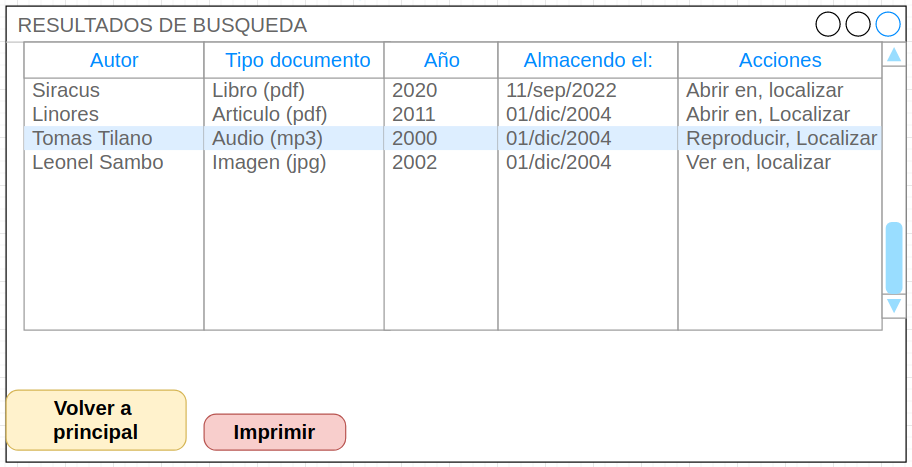
\includegraphics[scale=0.50]{images/resultadoBusqueda1}
	\caption{Resultado ¨de la busqueda}
\end{figure}

\begin{figure}
	\centering
	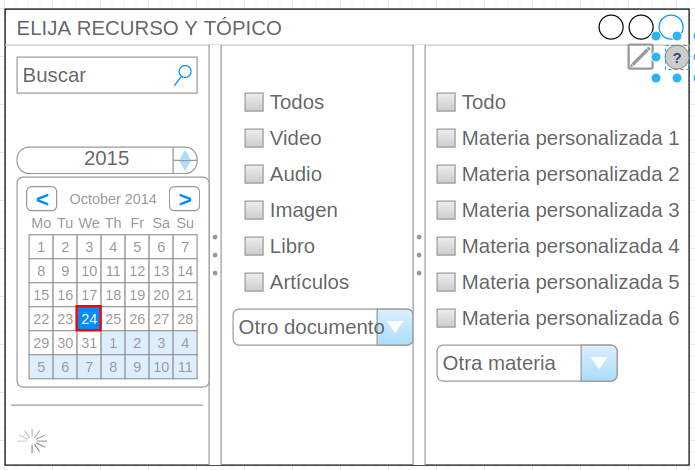
\includegraphics[scale=0.5]{images/buscador1}
	\caption{Pantalla principal de busqueda}
\end{figure}


\section{Diseño de Entrada efectiva}
El ingreso es mayormente de forma automática usando los metadatos de los objetos. 
\begin{figure}
	\centering
	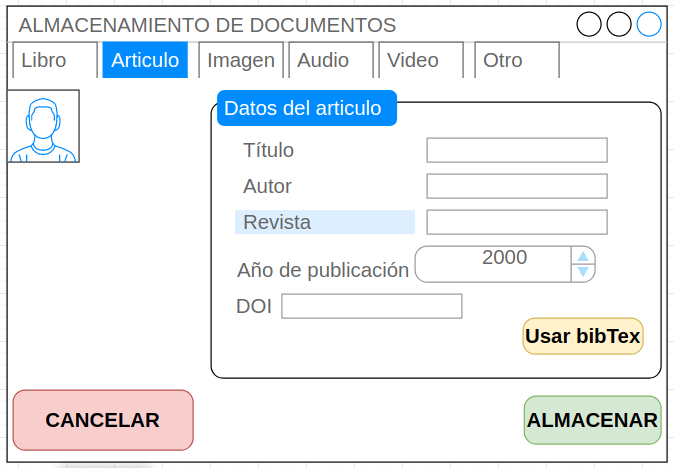
\includegraphics[scale=0.5]{images/almacenamientoDato1}
	\caption{Almacenamiento de artículos}
\end{figure}

%Un \textbf{reporte} es un docomento de negocios que contiene unicamente un dato predefinido.



